\begin{question}
Given the historical series of three stock prices in the file \href{https://raw.githubusercontent.com/matteosan1/finance_course/master/input_files/historical.csv}{historical.csv} compute the 1-day 95\% VaR and the corresponding Expected shortfall for a portfolio consisting of 40 FOX shares, 35 ABC shares and 25 CBS shares. 

\noindent\textbf{Hint:} when simulating the historical scenarios take care of possible NaN values in the series.
\end{question}

\cprotEnv\begin{solution}
\begin{ipython}
import pandas as pd
import numpy as np

df = pd.read_csv("historical.csv", index_col='date')
w = np.array([0.4, 0.25, 0.35])

df['P'] = df[['FOX', 'CBS', 'ABC']].dot(w)
df = df.pct_change()
df.dropna(inplace=True)
print (df.head())
\end{ipython}
\begin{ioutput}
                 FOX       CBS       ABC         P
date                                              
2018-03-26  0.013858 -0.012607  0.011189  0.006395
2018-03-23 -0.030891 -0.046818 -0.010830 -0.024072
2018-03-22  0.020592  0.020093  0.011543  0.015722
2018-03-21  0.003317  0.012137  0.052941  0.031266
2018-03-20 -0.003306 -0.011991 -0.003464 -0.005276
\end{ioutput}
\begin{ipython}
from numpy.random import seed, choice
from numpy import percentile
from finmarkets import var_discrete, es_discrete
 
var = var_discrete(df, 0.95, 'P')
es = es_discrete(df, 0.95, 'P')

print (f"VaR: {var:.4f}")
print (f"ES: {es:.4f}")
\end{ipython}
\begin{ioutput}
VaR: 0.0173
ES: 0.0232
\end{ioutput}
\begin{figure}[htbp]
\centering
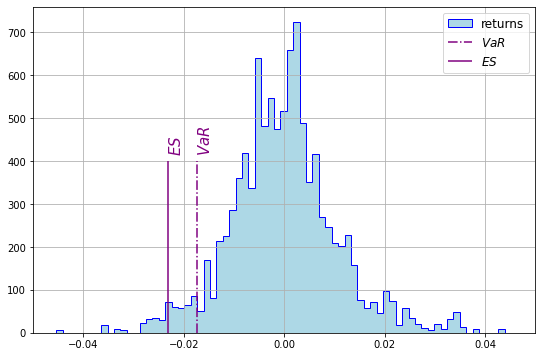
\includegraphics[width=0.7\linewidth]{figures/hist_var_ex}
\end{figure}
\end{solution}

\begin{question}
You have a 3-years call with strike 110 EUR. The underlying initial price is 105 EUR with a volatility of 0.15. The risk-free rate is 0.03 flat.
Compute the CVA of the contract assuming a recovery rate of 40\% and default probabilities for the underlying of 10\%, 20\% and 30\% for first, second and third year respectively.
\end{question}

\cprotEnv\begin{solution}
Below are shown ten realizations of the underlying price.

\begin{figure}[htbp]
\centering
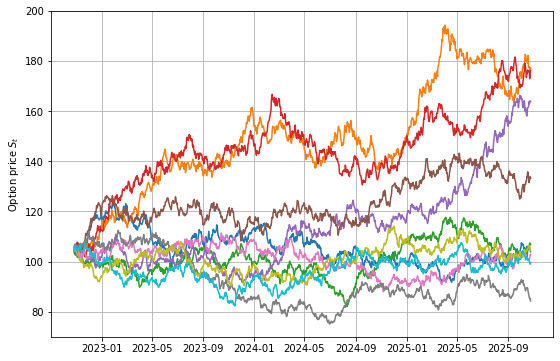
\includegraphics[width=0.7\linewidth]{figures/underlying_simulation}
\end{figure}

This implementation is not optimized in terms of speed, indeed it takes about 2 minutes to run 500 simulations.
A different approach, fully exploiting \texttt{numpy.array}s, could allow to shrink the execution time by a factor of 200.

\begin{ipython}
from datetime import date
from dateutil.relativedelta import relativedelta
from finmarkets import CreditCurve, call
from scipy.stats import norm
import numpy as np
import time

K = 110
sigma = 0.15
r = 0.03
T = 3
steps = 365*T
dt = 1/365
R = 0.4
Q = [0.9, 0.8, 0.7]
S0 = 105

obs_date = date.today()
dates = [obs_date + relativedelta(years=i+1) for i in range(T)]
cc = CreditCurve(obs_date, dates, Q)
t1 = time.time()
scenarios = 500
St = np.zeros(shape=(steps, scenarios))
St[0, :] = S0
ndps = np.zeros(shape=(steps,))
for i in range(1, steps):
    St[i, :] = St[i-1, :] * np.exp((r - 0.5 * sigma**2) * dt \
        + sigma* np.sqrt(dt) * norm.rvs(size=scenarios))
    ndps[i] = cc.ndp(obs_date+relativedelta(days=i-1)) - \
        cc.ndp(obs_date+relativedelta(days=i))

ts = [f"{t}y" for t in np.arange(T-dt, 0, -dt)]
cvas = np.zeros(shape=(steps, scenarios))
for s in range(scenarios):
    for j in range(len(ts)):
        cvas[j, s] = call(St[j, s], K, r, sigma, ts[j])*(1-R)*ndps[j]
cvas = np.sum(cvas, axis=0)
print (np.mean(cvas))
print (time.time() - t1)
\end{ipython}
\begin{ioutput}
2.464147656202549
129.0265169143676
\end{ioutput}
\end{solution}

\begin{question}
\label{ex:credit_var}
Consider a 1-years call with strike 110 EUR. The underlying initial price is 100 EUR with a volatility of 0.50. The risk-free rate is 0.03 flat. Compute the 99.9\% Credit VaR assuming a recovery rate of 40\% and default probabilities for the underlying of 30\% within next year.
\end{question}

\cprotEnv\begin{solution}

In order to increase the number of simulations the implemented code fully uses \texttt{numpy.array}.

\begin{ipython}
import numpy as np
from datetime import date
from dateutil.relativedelta import relativedelta
from finmarkets import CreditCurve
from scipy.stats import norm


K = 110
sigma = 0.50
r = 0.03
T = 1
steps = 365*T
dt = 1/365
R = 0.4
S0 = 100

obs_date = date.today()
cc = CreditCurve(obs_date, [obs_date + relativedelta(years=1)], [0.7])
scenarios = 10000
St = np.zeros(shape=(steps, scenarios))
St[0, :] = S0
ndps = np.zeros(shape=(steps,))
for i in range(1, steps):
    St[i, :] = St[i-1, :] * np.exp((r - 0.5 * sigma**2) * dt \
                                   + sigma* np.sqrt(dt) * norm.rvs(size=scenarios))
    ndps[i] = cc.ndp(obs_date+relativedelta(days=i)) - \
        cc.ndp(obs_date+relativedelta(days=i+1))

ts = [f"{t}y" for t in np.arange(T-dt, 0, -dt)]
EE = np.zeros(shape=(steps, scenarios))
for s in range(scenarios):
    EE[1:, s] = call(St[:-1, s], K, r, sigma, ts)*(1-R)*ndps[1:]
EE = np.sum(EE, axis=0)
print (f"Credit VaR: {np.percentile(EE, 99.9):.3f}")
\end{ipython}
\begin{ioutput}
Credit VaR: 26.281
\end{ioutput}

\begin{figure}[htbp]
\centering
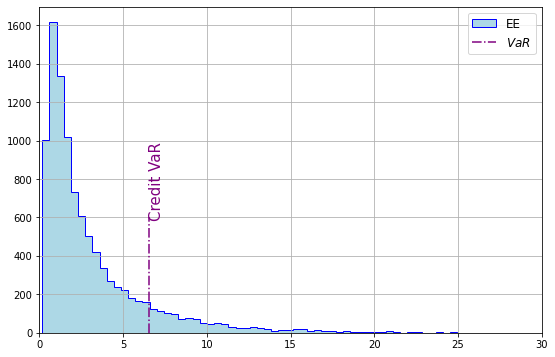
\includegraphics[width=0.7\linewidth]{figures/cr_var_ex}
\caption{Loss distribution to estimate Credit VaR measure of Ex.~\ref{ex:credit_var}.}
\end{figure}
\end{solution}





